\documentclass[10pt]{article}
\usepackage{tikz}
\usepackage[margin=0cm]{geometry}
\pagestyle{empty}

\begin{document}

\vspace*{\fill}
\begin{center}
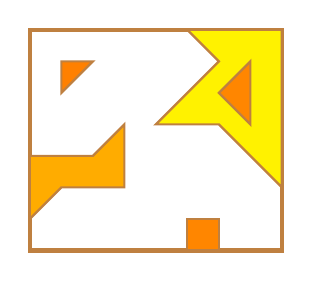
\begin{tikzpicture}[x=0.4cm, y=-0.4cm, thick, brown]
\draw[ultra thick] (0, 0) -- (8, 0) -- (8, 7) -- (0, 7) -- cycle;

% Depth 0
\filldraw[fill=orange!0!yellow] (5, 0) -- (8, 0) -- (8, 5) -- (6, 3) -- (4, 3) -- (6, 1) -- cycle;
\filldraw[fill=orange!100!yellow] (1, 1) -- (2, 1) -- (1, 2) -- cycle;
\filldraw[fill=orange!65!yellow] (3, 3) -- (3, 5) -- (1, 5) -- (0, 6) -- (0, 4) -- (2, 4) -- cycle;
\filldraw[fill=orange!95!yellow] (5, 6) -- (6, 6) -- (6, 7) -- (5, 7) -- cycle;
% Depth 1
\filldraw[fill=orange!95!yellow] (7, 1) -- (7, 3) -- (6, 2) -- cycle;
\end{tikzpicture}
\end{center}
\vspace*{\fill}

\end{document}
